\documentclass{beamer}

% Theme selection
%\usetheme{metropolis} % A clean, professional theme
\usetheme{moloch}% modern fork of the metropolis theme
%\setbeamertemplate{frame footer}{\insertshortauthor~(\insertshortinstitute)}

%\setbeamerfont{page number in head/foot}{size=\tiny}
\setbeamercolor{footline}{fg=gray}
%\usecolortheme{beaver} % Good color scheme for readability
%\usefonttheme{structuresmallcapsserif} % Consistent font

\usepackage[style=authortitle,backend=bibtex]{biblatex}
\addbibresource{Compressive_Sensing_Report.bib} 


% Packages
%\usepackage[utf8]{inputenc}
\usepackage{amsmath, amssymb}
\usepackage{graphicx}
\usepackage{hyperref}
\usepackage{subcaption} % For subfigure environment
% Removed stackengine and parskip as they are less common in Beamer and can cause formatting issues.
% If you need specific vertical spacing, use vspace.

\usepackage{listings} % For code snippets
\usepackage{color} % Needed for defining colors

% Color definitions (already in your preamble, just ensuring they are here)
\definecolor{codegreen}{rgb}{0,0.6,0}
\definecolor{codegray}{rgb}{0.5,0.5,0.5}
\definecolor{codepurple}{rgb}{0.58,0,0.82}
\definecolor{backcolour}{rgb}{0.95,0.95,0.92}

% Listing style for code snippets (already in your preamble)
\lstdefinestyle{mystyle}{
    backgroundcolor=\color{backcolour},
    commentstyle=\color{codegreen},
    keywordstyle=\color{magenta},
    numberstyle=\tiny\color{codegray},
    stringstyle=\color{codepurple},
    basicstyle=\ttfamily\footnotesize,
    breakatwhitespace=false,
    breaklines=true,
    captionpos=b,
    keepspaces=true,
    numbers=left,
    numbersep=5pt,
    showspaces=false,
    showstringspaces=false,
    showtabs=false,
    tabsize=2
}
\lstset{style=mystyle}

% Title page details (as in your preamble)
\title{Compressive Sensing with Applications to Near-Field to Far-Field Antenna Pattern Extrapolation}
\subtitle{Semester Project}
\author{Jonas Thalmeier}
\institute{Supervised by Prof. Dirk Slock, Dr. Zilu Zhao, Dr. Fangqing Xiao}
\date{20/06/2025}

\begin{document}

% Title Slide
\begin{frame}
    \titlepage
\end{frame}

% Table of Contents
\begin{frame}
    \frametitle{Table of Contents}
    \tableofcontents
\end{frame}

% --- SECTION: Introduction ---
\section{Introduction}

\begin{frame}
    \frametitle{Motivation: Antenna Measurement Challenges}
    \begin{itemize}
        % \item \textbf{Precise Antenna Characterization:} Critical for performance.
        \item \textbf{Near-Field (NF) to Far-Field (FF) Transformation:}
        \begin{itemize}
            \item Necessary because direct FF measurements are often impractical (requires very large anechoic chambers).
            \item NF measurements are taken close to the antenna and then transformed to FF.
            \item Precise NF characterization necessary
        \end{itemize}
        \item \textbf{Challenges:} %Reducing the number of required near-field measurements without degrading far-field prediction accuracy.
        \begin{itemize}
        		\item \textbf{Truncation:} Some areas might be inaccessible
        		\item \textbf{Measurement Grid Density:} Acquiring measurement over a dense grid is time consuming
        \end{itemize}
    \end{itemize}
\end{frame}

\begin{frame}
    \frametitle{Project Objectives and Approach}
    \begin{itemize}
        \item \textbf{Main Objective:} Apply Compressive Sensing (CS) to near-field antenna measurements to enable precise FF extrapolation with relatively few measurements.
        \item \textbf{Approach:}
        \begin{itemize}
            \item Understand, Implement and evaluate various Sparse Bayesian Learning (SBL) algorithms (EM, CoFEM, Tipping's FML) for antenna pattern expansion.
            \item Leverage the Spherical Wave Expansion (SWE) for antenna field representation.
        \end{itemize}
        \item \textbf{Tools Used:} Python for algorithm implementation, MATLAB for Antenna simulation.
    \end{itemize}
\end{frame}

% --- SECTION: Theoretical Foundations ---
\section{Theoretical Foundations}

\begin{frame}
    \frametitle{Compressive Sensing Basics}
    \begin{itemize}
        \item \textbf{Core Idea:} Recovering sparse signals from a small number of linear measurements.
        \item \textbf{Key Concepts:}
        \begin{itemize}
            \item \textbf{Sparsity:} The signal of interest can be represented sparsely in some basis.
            \item \textbf{Undersampling:} Measurements $N$ are significantly fewer than signal dimension $D$ ($N \ll D$).
            %\item \textbf{Restricted Isometry Property (RIP):} A property of the sensing matrix $\Phi$ that ensures stable recovery.
        \end{itemize}
        \item \textbf{Mathematical Formulation:}
        \begin{equation*}
            \mathbf{t} = \Phi \mathbf{w} + \mathbf{e}
        \end{equation*}
        Where $\mathbf{t}$ is the measurement vector, $\Phi$ is the sensing matrix, $\mathbf{w}$ is the sparse signal, and $\mathbf{e}$ is noise.
    \end{itemize}
\end{frame}

\begin{frame}
    \frametitle{Sparse Bayesian Learning (SBL)}
    \begin{itemize}
        \item \textbf{Core Idea:} Inducing sparsity in weight vectors by optimizing a parameterized Gaussian prior over the signal weights.
        \item \textbf{Observation Model:} $\mathbf{t} = \Phi \mathbf{w} + \boldsymbol{\epsilon}$, where $\boldsymbol{\epsilon} \sim \mathcal{N}(0, \sigma^2 \mathbf{I})$.
        \item \textbf{Prior Distribution for $\mathbf{w}$:} $p(w_i;\gamma_i) \sim \mathcal{N}(0,\gamma_i)$
        \item \textbf{Inference:} Hyperparameters $\boldsymbol{\gamma}$ and $\sigma^2$ are inferred e.g. via Type-II Maximum Likelihood (evidence maximization):
        \begin{equation}
        	\hat{\mathbf{\gamma}},\mathbf{\sigma}^2= \arg\max p(t\mid\mathbf{\gamma},\mathbf{\sigma}^2)
        \end{equation}
    \end{itemize}
\end{frame}

% --- SECTION: SBL Algorithms Implemented ---
\section{SBL Algorithms Implemented}

\subsection{Expectation-Maximization (EM)}
\begin{frame}
    \frametitle{EM Algorithm for SBL \footcite{wipf2004sparse}}
    \begin{itemize}
        \item \textbf{Overview:} An iterative algorithm for estimating the sparse weights $\mathbf{w}$ and hyperparameters $\boldsymbol{\gamma}$, $\sigma^2$.
        \item \textbf{Iterative Steps:}
        \begin{itemize}
            \item \textbf{E-step:} Compute posterior distribution $p(\mathbf{w} \mid \mathbf{t}, \boldsymbol{\gamma}, \sigma^2)$, specifically its mean ($\boldsymbol{\mu}_w$) and covariance ($\boldsymbol{\Sigma}_w$).
            \item \textbf{M-step:} Update hyperparameters $\boldsymbol{\gamma}$ and $\sigma^2$ using the computed posterior statistics.
        \end{itemize}
        \item \textbf{Challenges:}
        \begin{itemize}
            \item Computationally expensive due to $D \times D$ matrix inversion in each iteration: $\boldsymbol{\Sigma}_w = \left( \beta \Phi^\top \Phi + \mathrm{diag}(\boldsymbol{\gamma}^{-1}) \right)^{-1}$.
            \item Robust performance in Gaussian measurement systems, but showed instability for complex-valued (e.g., Fourier) data.
        \end{itemize}
    \end{itemize}
\end{frame}

\subsection{Covariance-Free Expectation Maximization (CoFEM)}
\begin{frame}
    \frametitle{CoFEM Algorithm \footcite{lin2022covariance}}
    \begin{itemize}
        \item \textbf{Motivation:} Address the high computational cost of the EM algorithm.
        \item \textbf{Key Idea:} Avoids explicit computation of the full posterior covariance matrix $\boldsymbol{\Sigma}_w$.
        \item \textbf{Approach:}
        \begin{itemize}
            \item Estimates required posterior statistics (e.g., diagonal elements of $\boldsymbol{\Sigma}_w$) by solving linear systems.
            \item Uses techniques like Rademacher probe vectors for approximation.
        \end{itemize}
        \item \textbf{Performance:}
        \begin{itemize}
            \item Achieved significant runtime reduction compared to standard EM, especially for larger $D$.
            \item For $N=500, D=1500$, CoFEM runtime was 98.4s vs. EM's 146.6s.
            \item Reconstruction accuracy was comparable to EM for Gaussian matrices.
        \end{itemize}
    \end{itemize}
\end{frame}

\begin{frame}
    \frametitle{EM vs. CoFEM: Runtime and Accuracy}
    \begin{columns}
        \begin{column}{0.48\textwidth}
            \textbf{Runtime Comparison:}
            \begin{itemize}
                \item CoFEM is faster, especially for increasing $N$.
                \item Still, limitations for very large-scale problems.
            \end{itemize}
            \begin{figure}[h!]
                \centering
                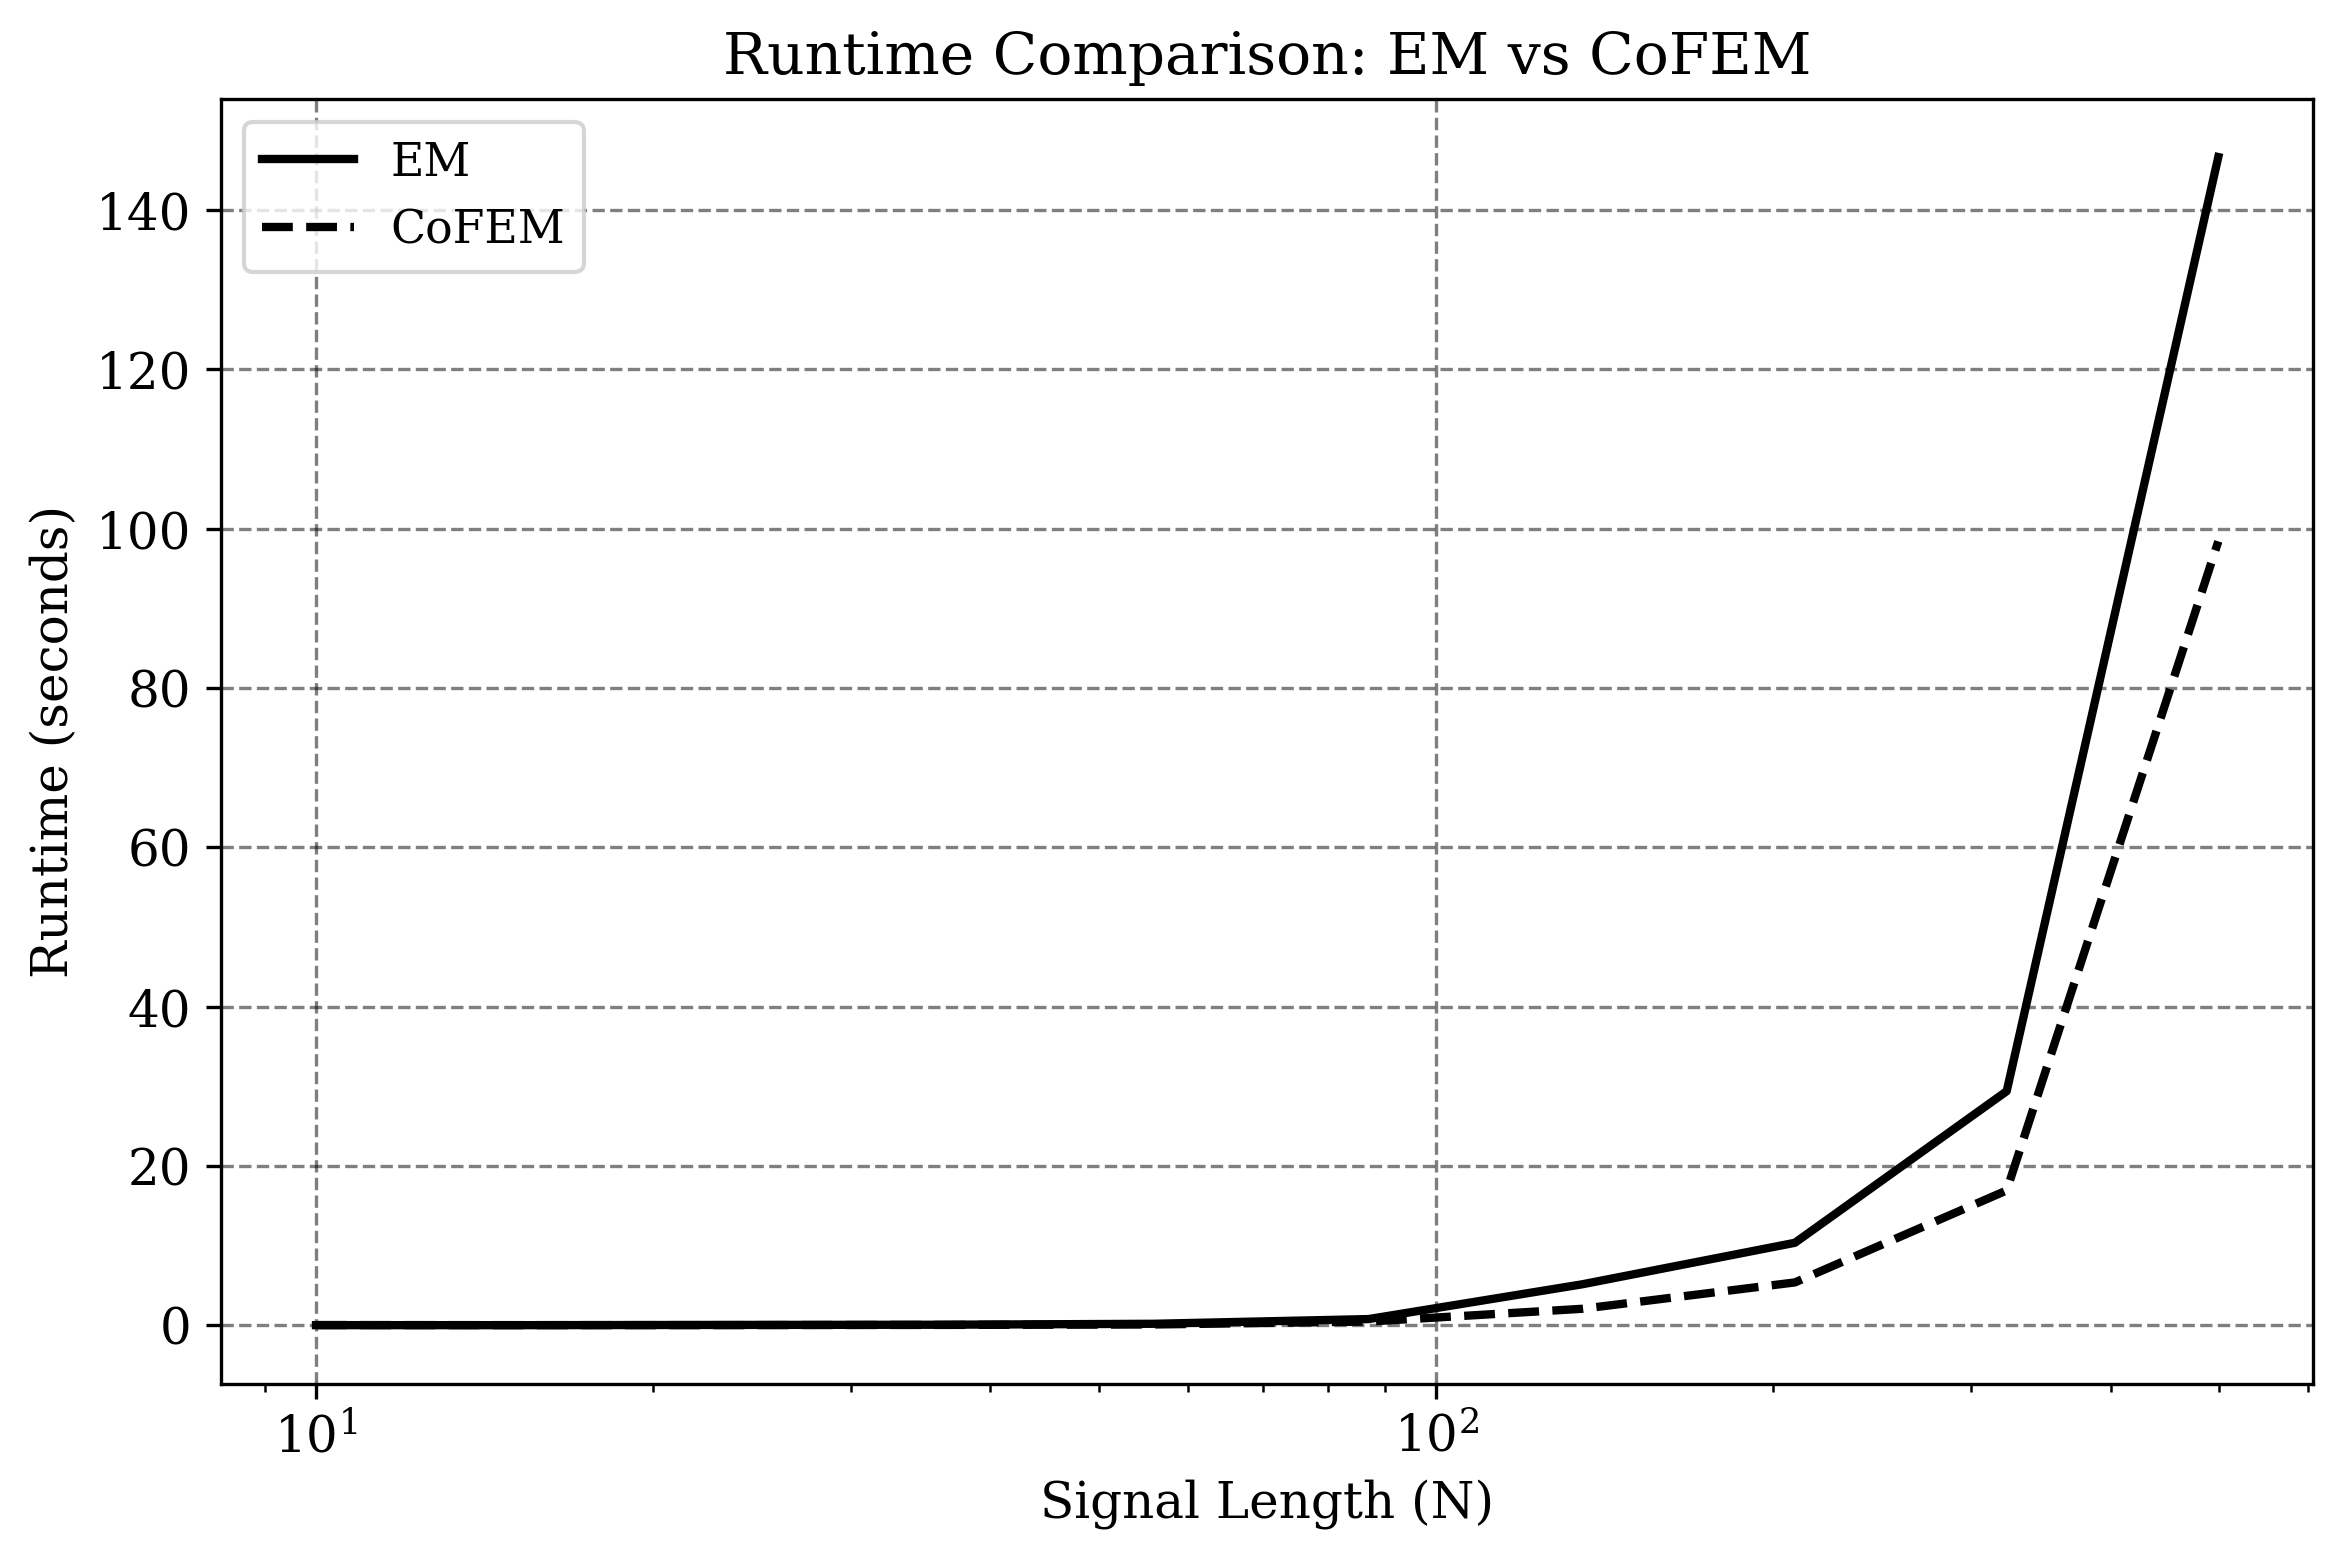
\includegraphics[width=\textwidth]{Figures/runtime_comp.png}
                \caption{Runtime of EM and CoFEM for increasing $N$ ($D=3N$).}
            \end{figure}
        \end{column}
        \begin{column}{0.48\textwidth}
            \textbf{Accuracy (Gaussian Matrices):}
            \begin{itemize}
                \item Both EM and CoFEM showed similar accuracy.
                \item CoFEM with unknown noise variance performed well.
            \end{itemize}
            \begin{figure}[h!]
                \centering
                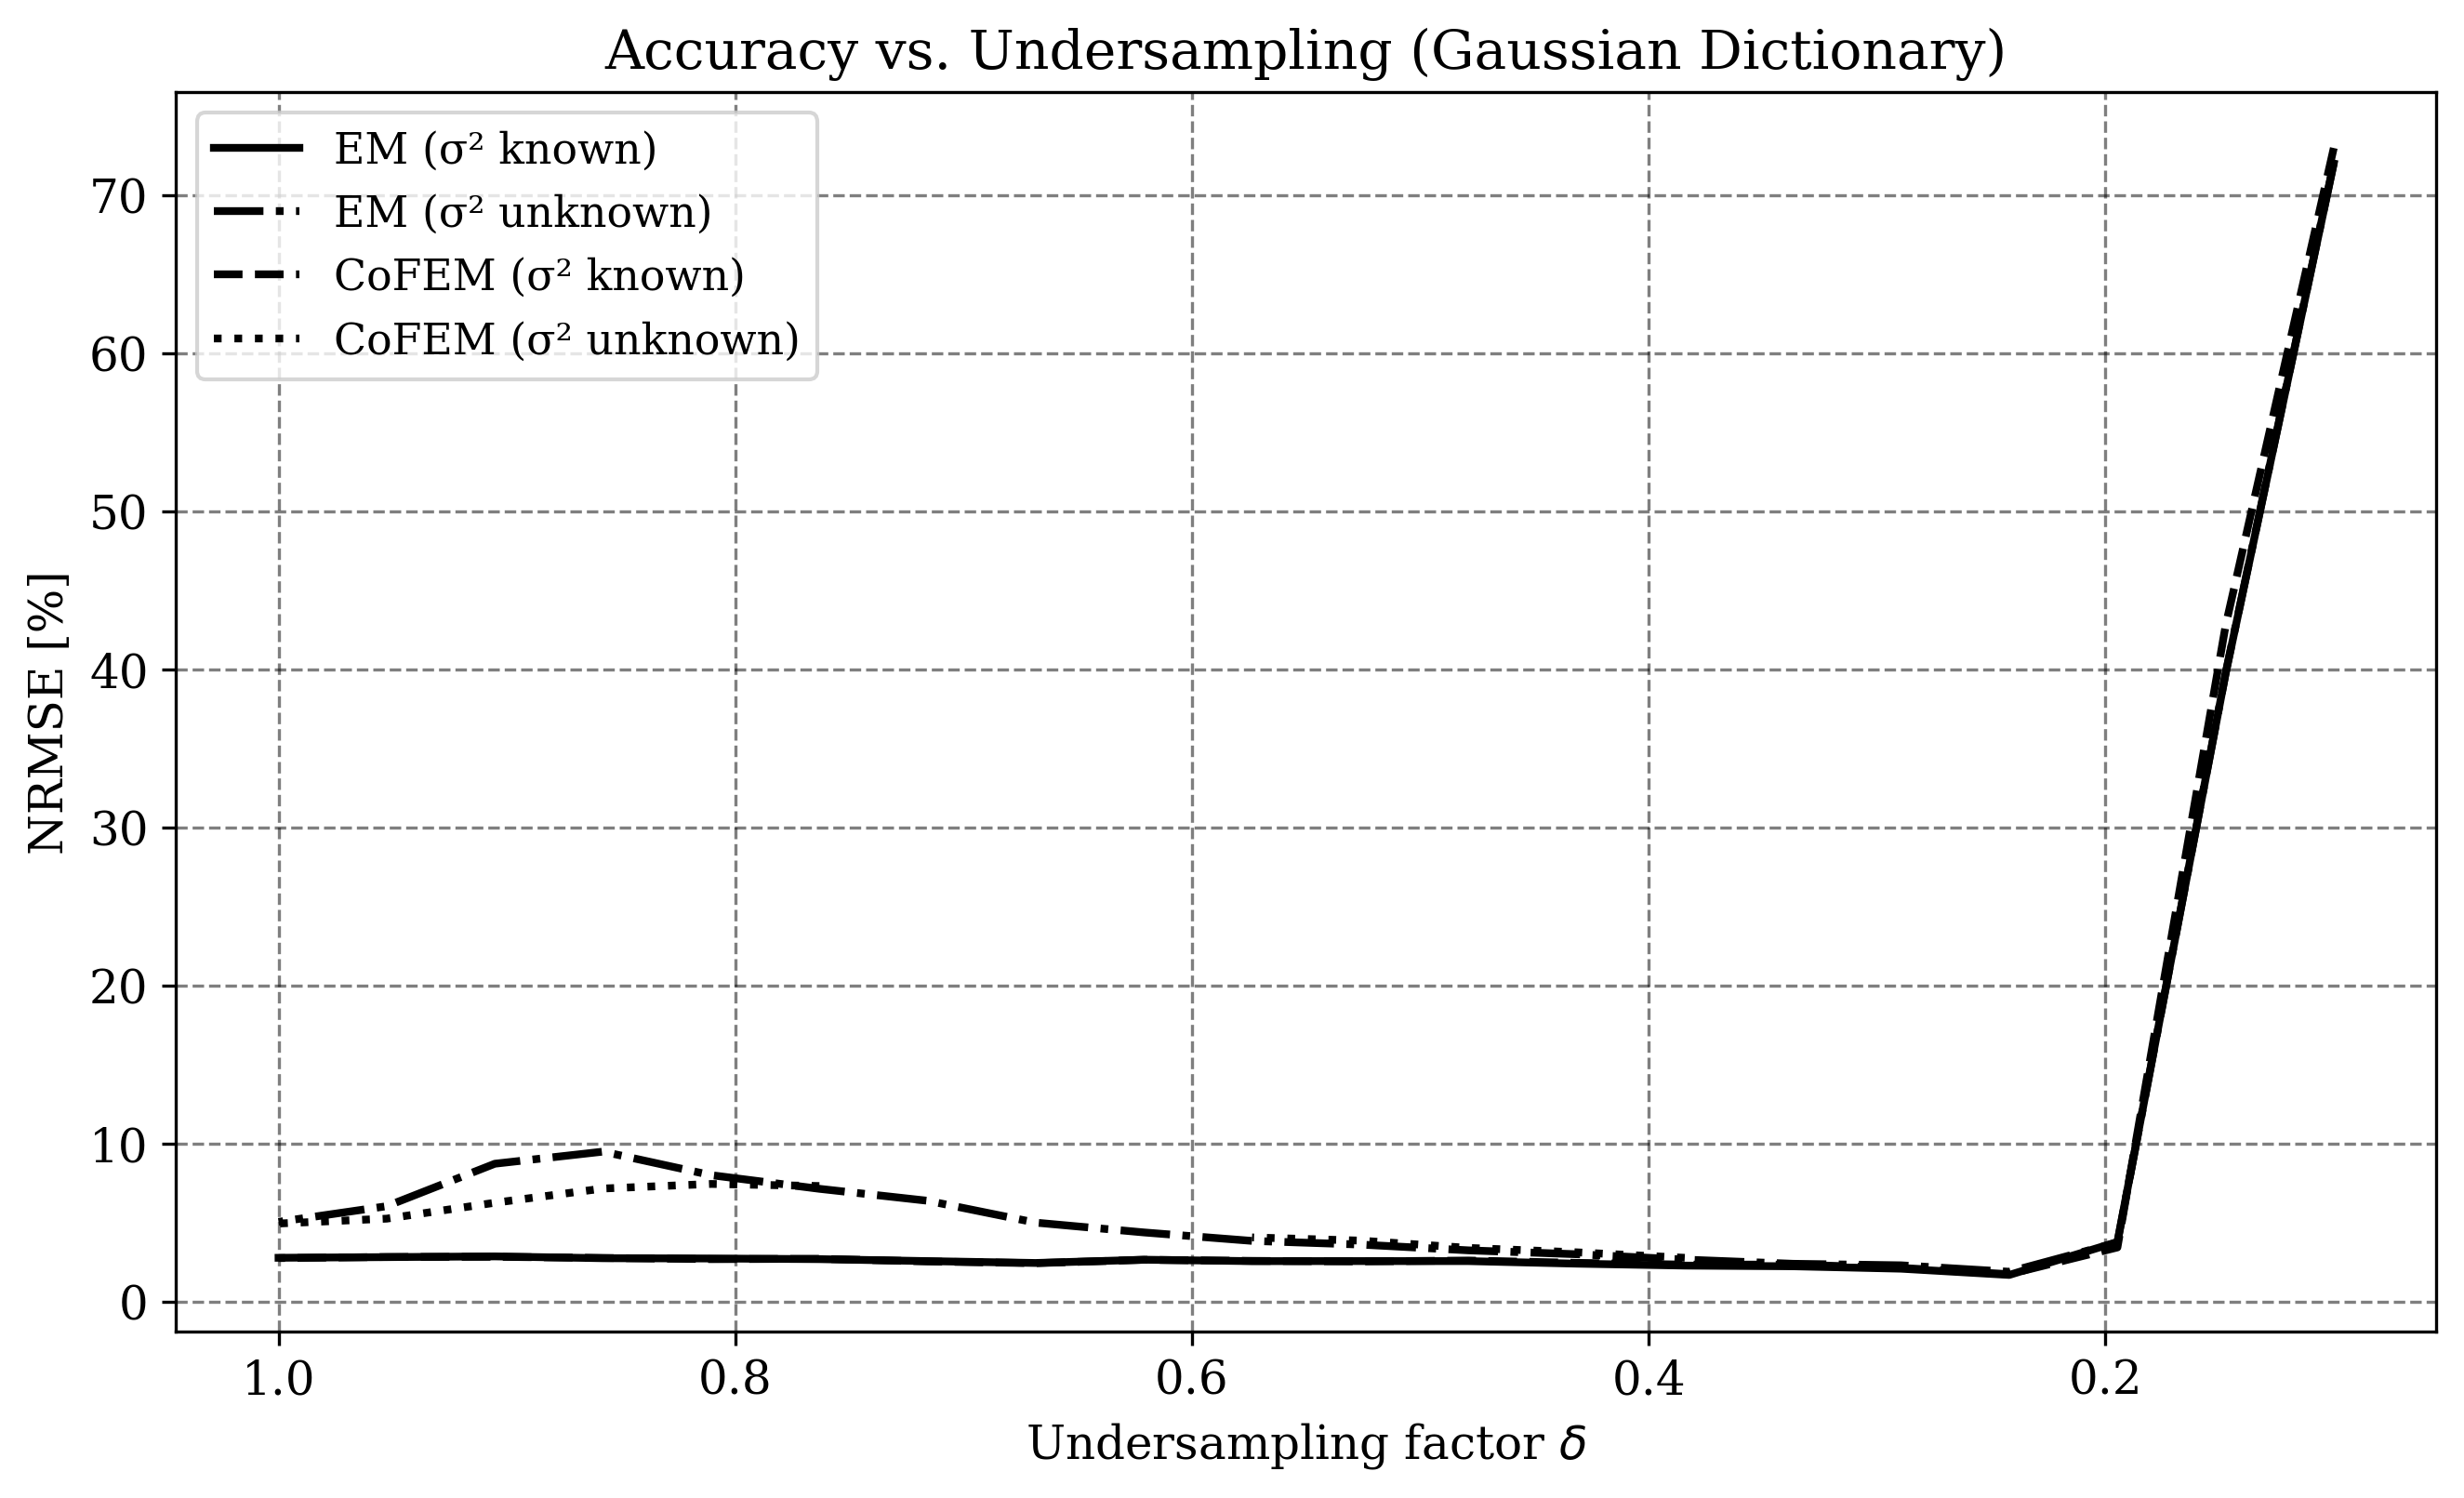
\includegraphics[width=\textwidth]{Figures/accuracy_vs_undersampling_EMCoFEM.png}
                \caption{NRMSE vs. undersampling factor $\delta$ for EM and CoFEM (Gaussian $\Phi$).}
            \end{figure}
        \end{column}
    \end{columns}
    % Removed \justifying as it was causing an error and isn't typically used here.
    \textbf{Note:} EM/CoFEM showed instability and unreliable results with complex-valued (Fourier) matrices, leading to discontinuation of their use for that specific application.
\end{frame}

\subsection{SURE \& Tipping's Fast Marginal Likelihood (FML) Algorithm}
\begin{frame}
    \frametitle{Stein's Unbiased Risk Estimate (SURE)}
    \begin{itemize}
        \item \textbf{Purpose:} Provides an unbiased estimate of the Mean Squared Error (MSE) or "risk" of an estimator, without needing to know the true signal \footcite{Tibshirani2015SteinS}.
        \item \textbf{SURE Formula for $\hat{\mu}$ as a function of $\mathbf{y}$ (measurements):}
        \begin{equation*}
            \widehat{R}(\hat{\boldsymbol{\mu}}(\mathbf{y})) = \|\mathbf{y} - \hat{\boldsymbol{\mu}}(\mathbf{y})\|_2^2 - n\sigma^2 + 2\sigma^2 \sum_{i=1}^n \frac{\partial \hat{\mu}_i(\mathbf{y})}{\partial y_i}
        \end{equation*}
        \item \textbf{Application in SBL:} Can be used to optimize hyperparameters (e.g., prior variances $\gamma_i$) by minimizing the SURE \footcite{slockSURE}.
        \item \textbf{Optimal Prior Variances:} $p_i = \lfloor|\hat{x}_i(0)|^2 - \sigma^2\rfloor_+$ (same result as Type II ML).
    \end{itemize}
\end{frame}

\begin{frame}
    \frametitle{Tipping's Fast Marginal Likelihood Algorithm \footcite{tipp2003fastsb}}
    \begin{itemize}
        \item \textbf{Connection to SURE:} While not directly using the SURE formula for optimization in its primary form, Tipping's FML effectively maximizes the marginal likelihood, which is was shown to have the same result as SURE approach.
        \item \textbf{Key Features:}
        \begin{itemize}
            \item \textbf{Sequential Basis Selection and Pruning:} Iteratively adds relevant basis functions and prunes irrelevant ones.
            \item \textbf{Efficient Hyperparameter Updates:} Based on closed-form solutions for Type II Maximum Likelihood.
        \end{itemize}
        \item \textbf{Advantages:}
        \begin{itemize}
            \item Explicit sparsity enforcement (many $\gamma_i$ driven to zero).
            \item Faster convergence compared to EM for many problems.
            \item More robust to choice of dictionary matrix (both Gaussian and complex-valued).
        \end{itemize}
    \end{itemize}
\end{frame}

\begin{frame}
    \frametitle{Tipping's FML Performance}
    \begin{itemize}
        \item \textbf{Robustness:} Consistent performance across both Gaussian and complex-valued (Fourier) systems.
        \item \textbf{Accuracy (Gaussian Systems):} Comparable to EM, with EM showing marginal improvements in some cases.
        \item \textbf{Key Finding (Complex-Valued Systems):}
        \begin{itemize}
            \item Tipping's method significantly outperformed its own performance in Gaussian systems when applied to complex-valued dictionaries.
            \item This indicates better adaptability and robustness to structured (non-i.i.d.) sensing matrices, which are common in real-world antenna problems.
        \end{itemize}
    \end{itemize}
    \begin{figure}[h!]
        \centering
        \begin{subfigure}[b]{0.48\textwidth}
            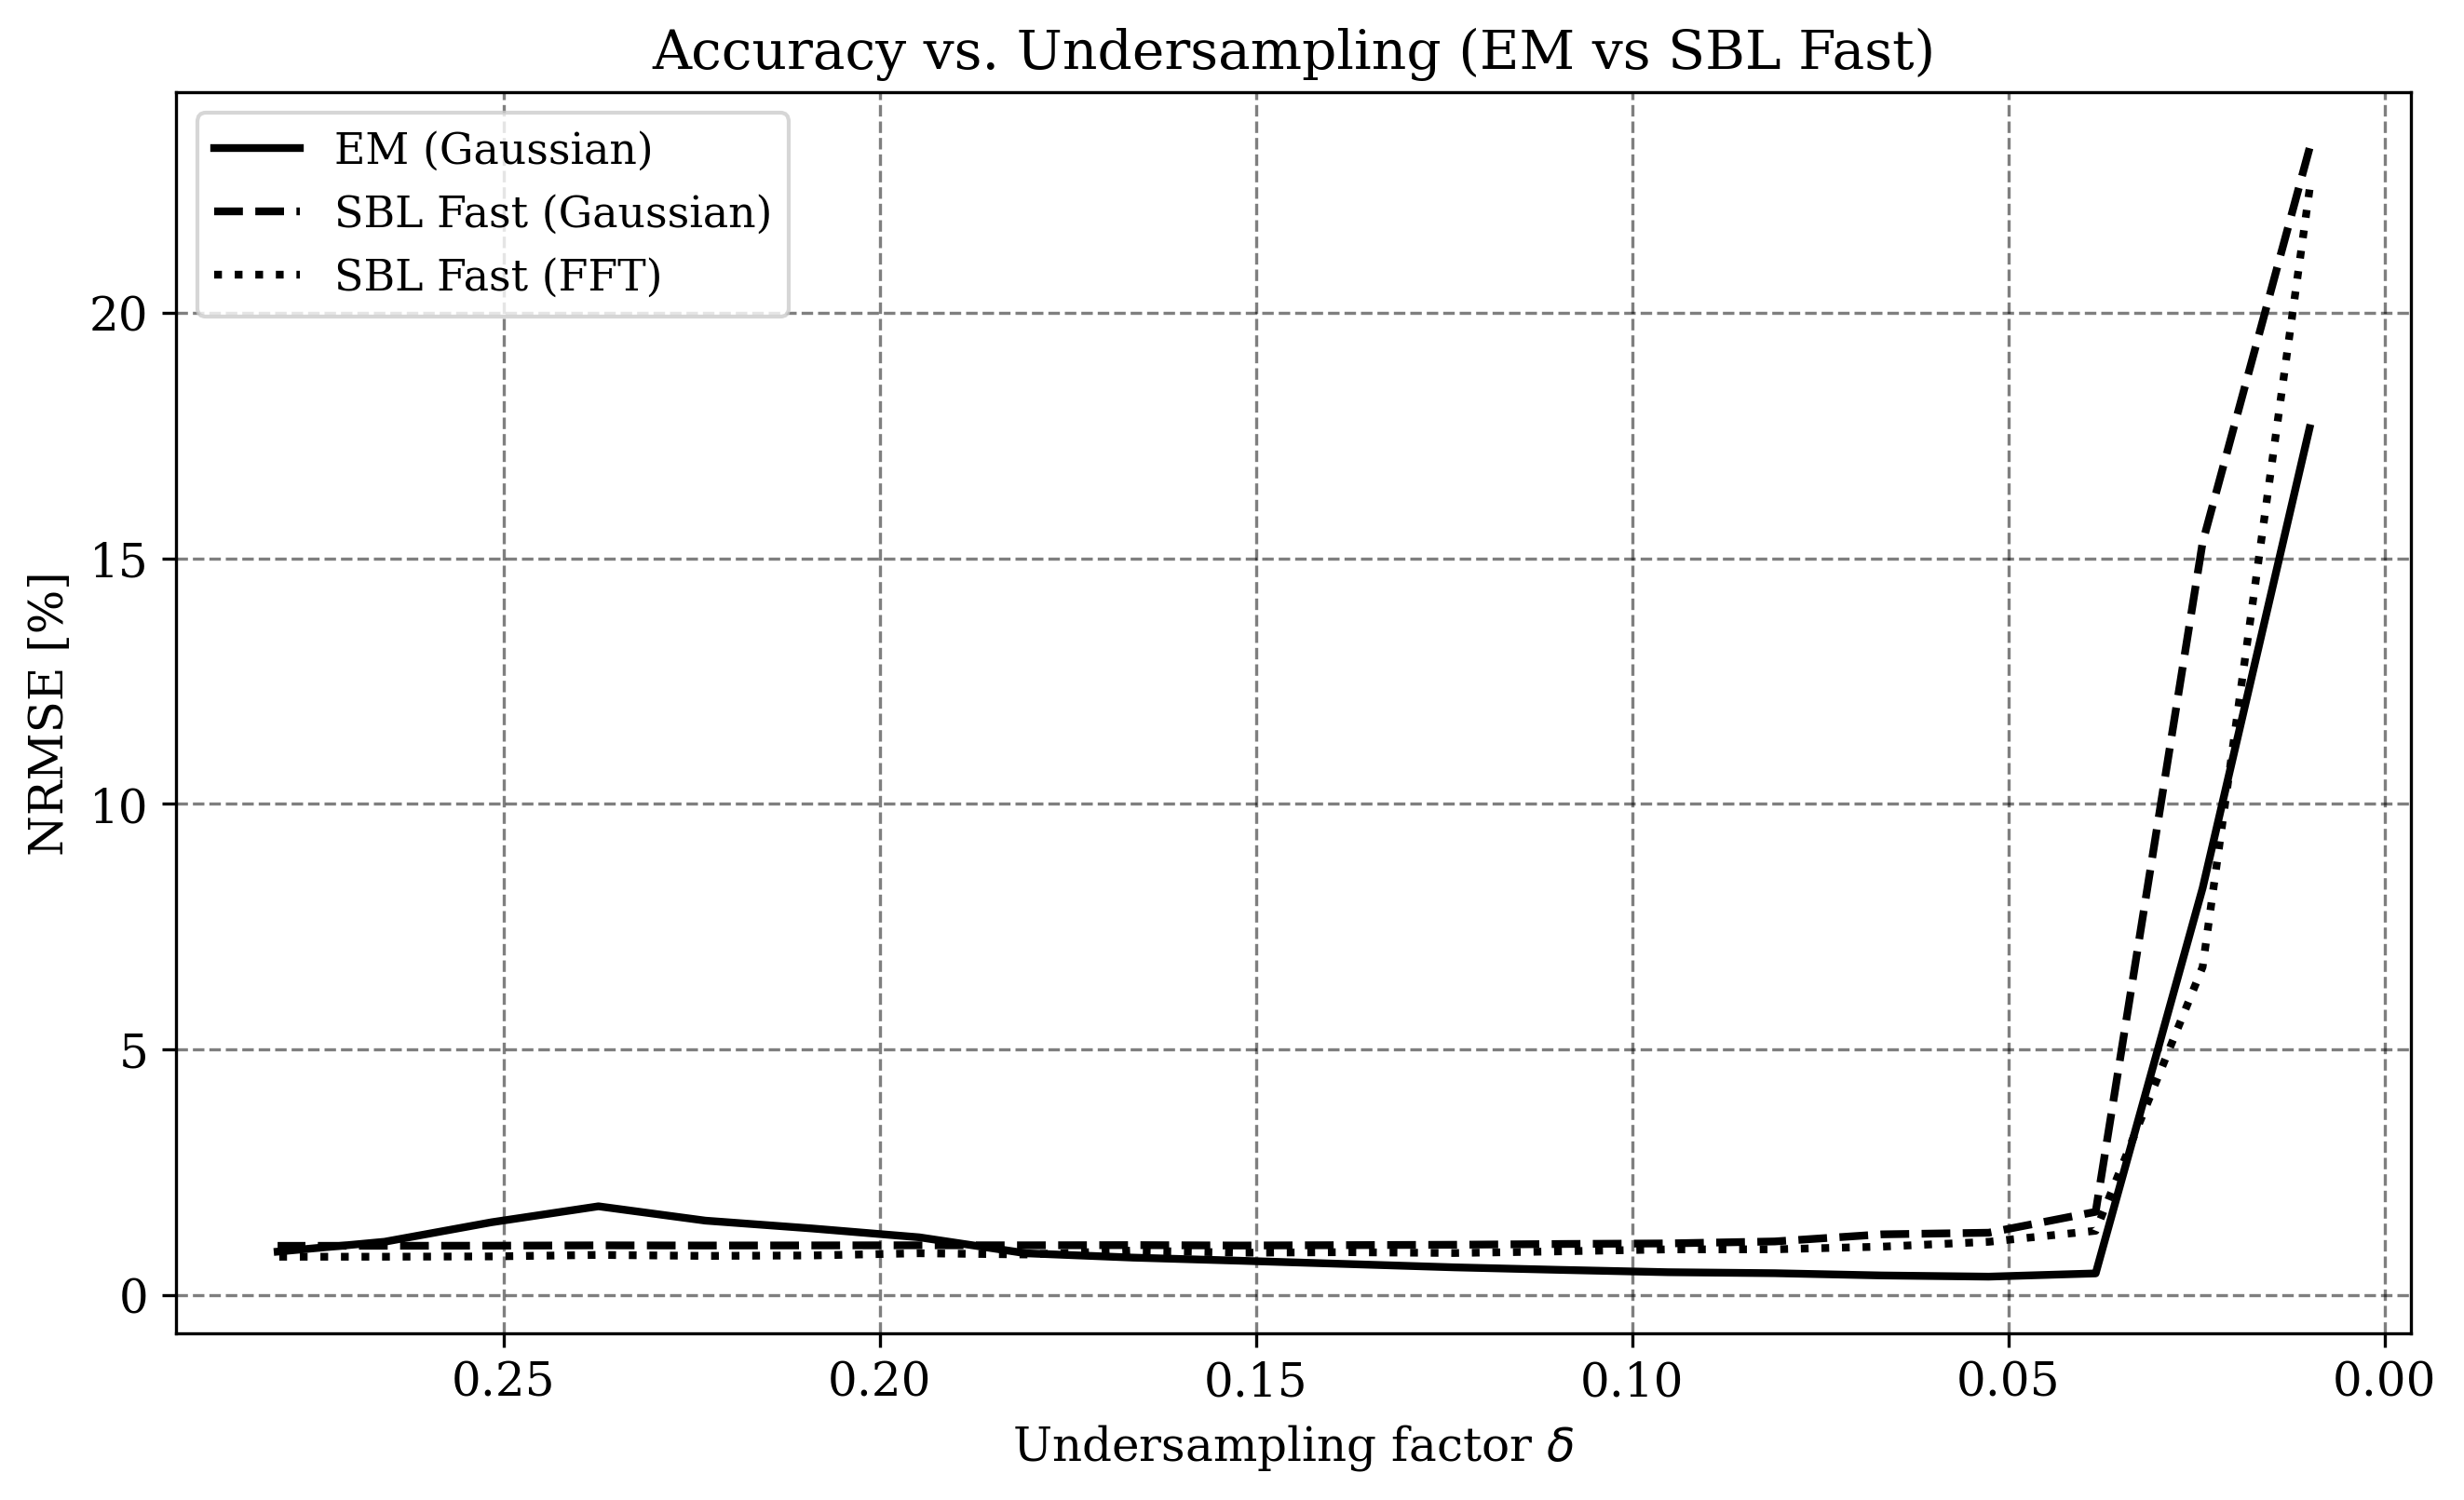
\includegraphics[width=\textwidth]{Figures/accuracy_vs_undersampling_EMvsSB_woEMFFT.png}
            \caption{NRMSE vs. undersampling factor $\delta$.}
        \end{subfigure}
        \hfill
        \begin{subfigure}[b]{0.48\textwidth}
            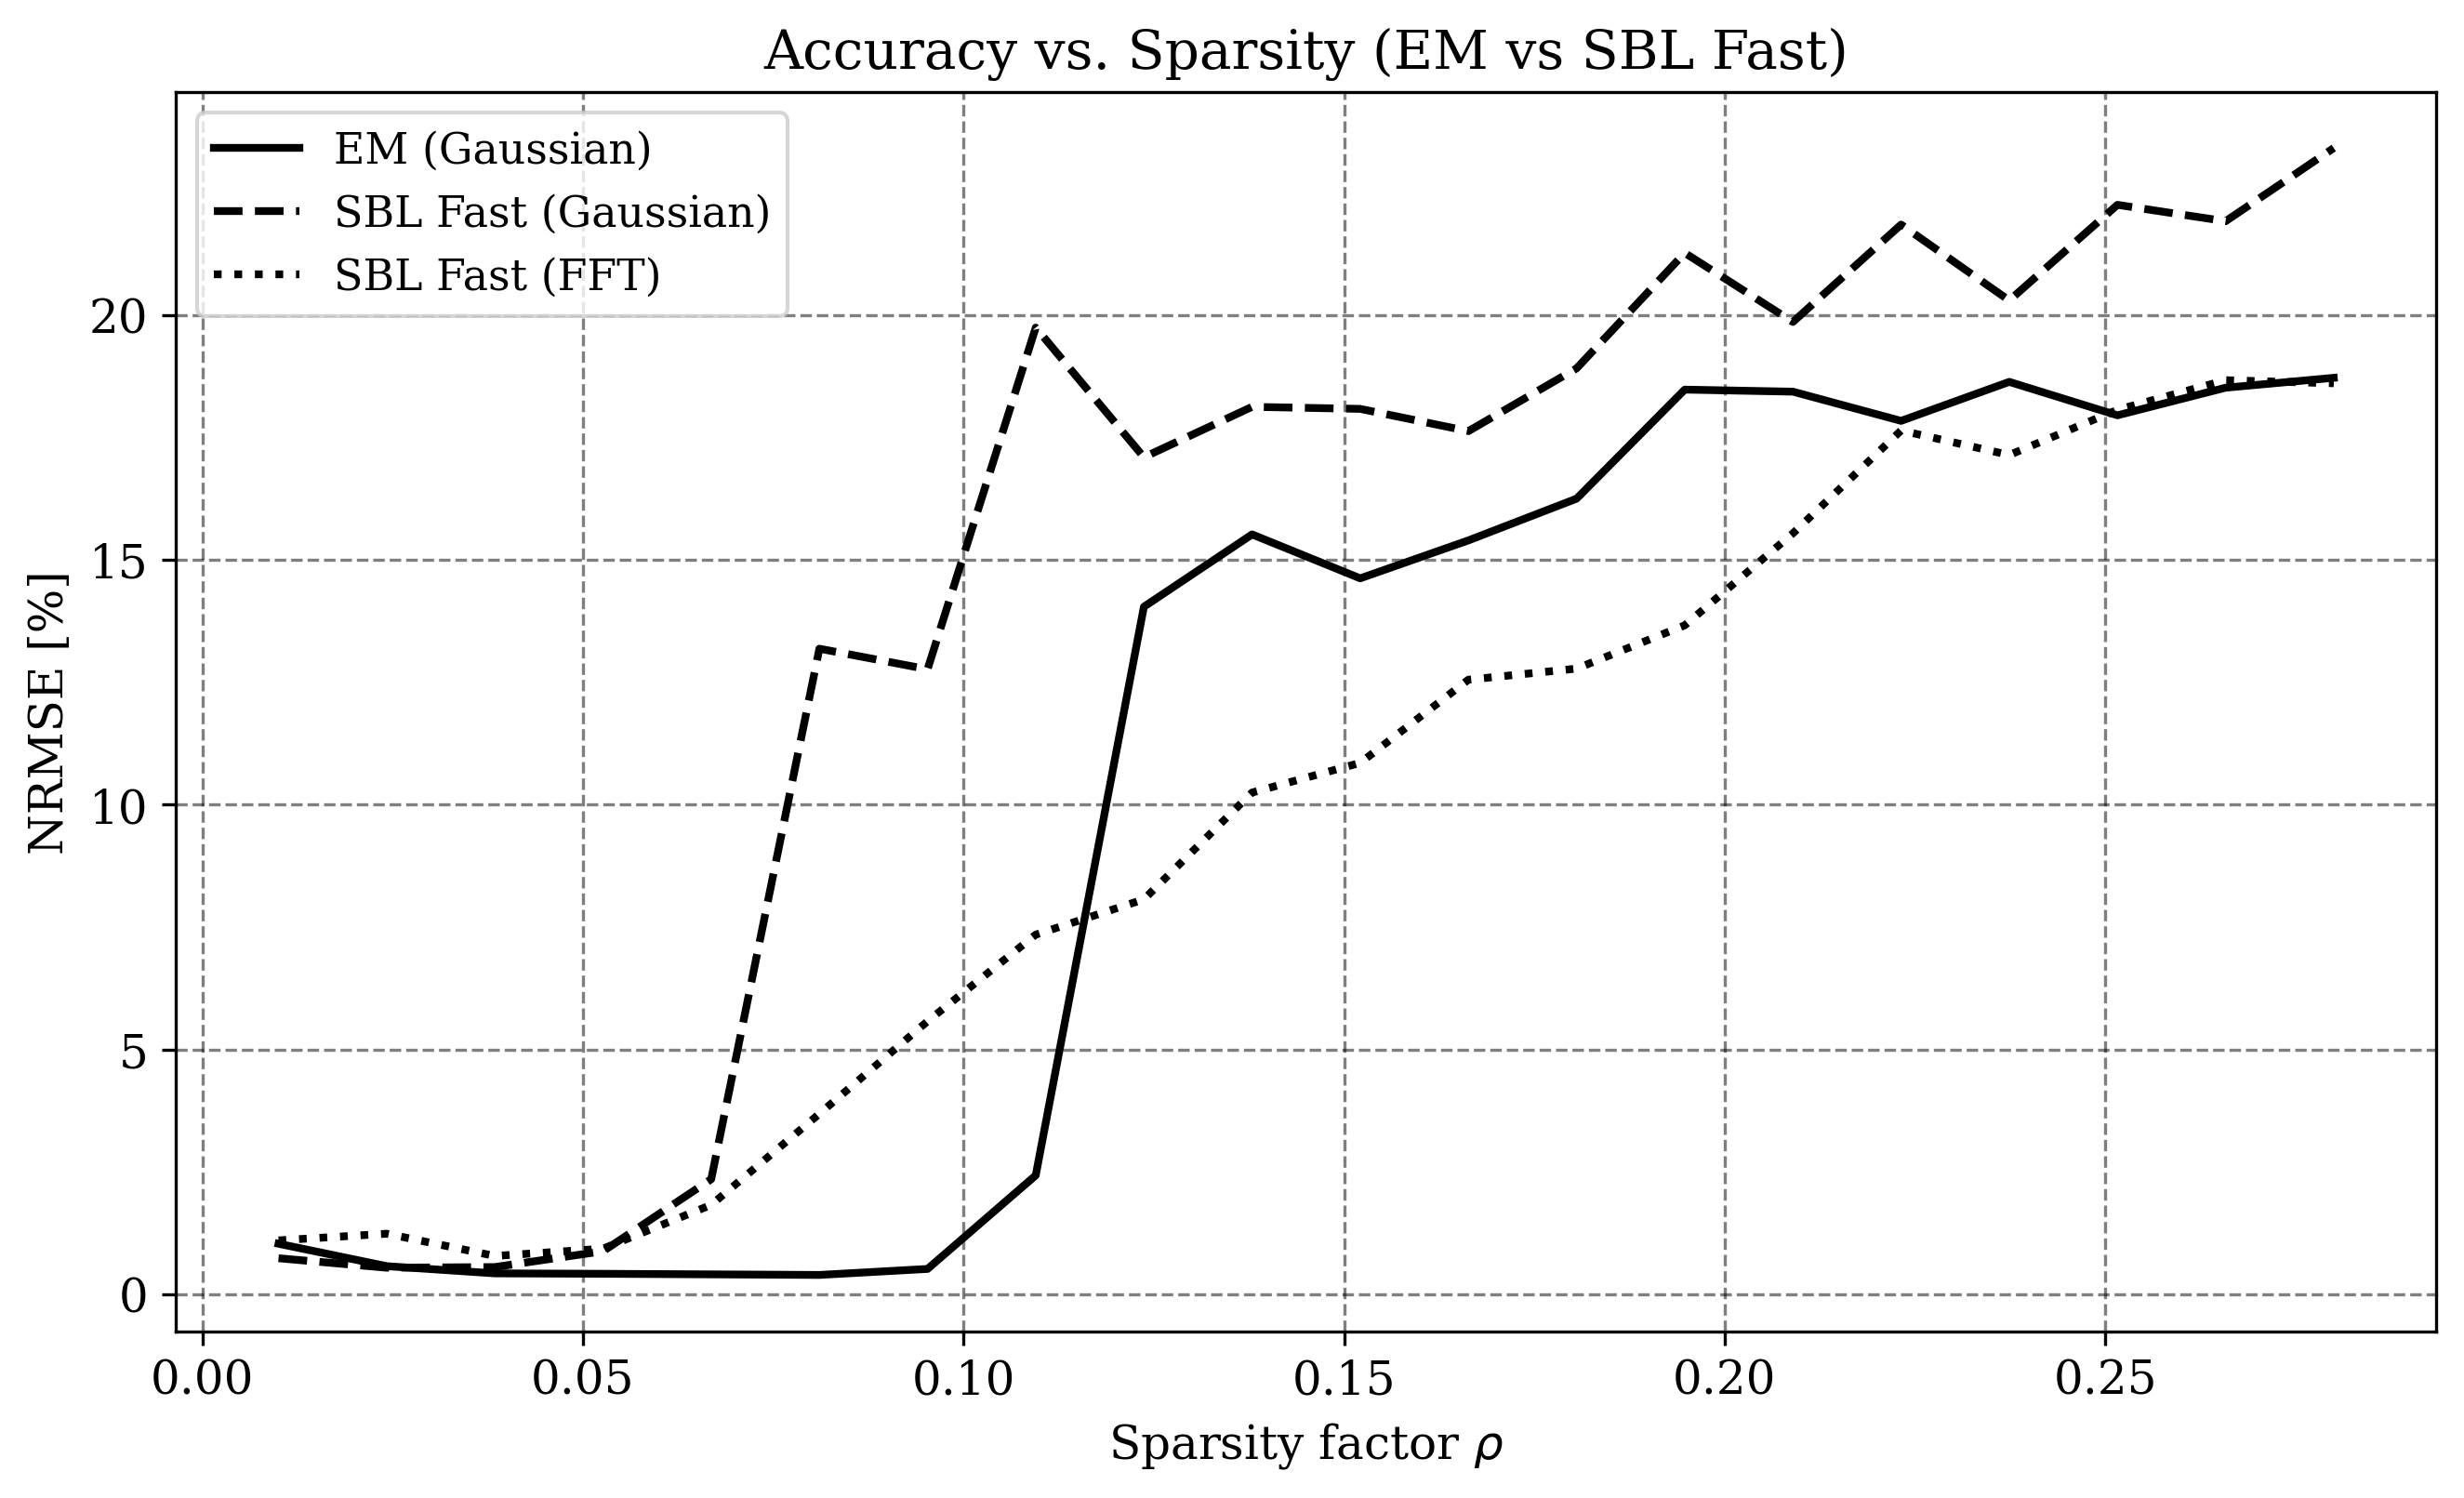
\includegraphics[width=\textwidth]{Figures/accuracy_vs_sparsity_EMvsSB_woEMFFT.png}
            \caption{NRMSE vs. sparsity ratio $\rho$.}
        \end{subfigure}
        \caption{Reconstruction accuracy for Tipping's FML algorithm (SB for Sparse Bayesian).}
    \end{figure}
\end{frame}

% --- SECTION: Spherical Wave Expansion (SWE) ---
\section{Spherical Wave Expansion (SWE)}

\begin{frame}
    \frametitle{Spherical Wave Functions \footcite{hansen1988spherical}}
    \begin{itemize}
        \item \textbf{Concept:} Any electromagnetic field in a source-free region can be expressed as a superposition of spherical vector wave functions.Therefore the electric field $\mathbf{E}(r, \theta, \phi)$ can be decomposed into spherical vector wave functions $\mathbf{F}_{smn}^{(c)}$.
        \item \textbf{Equation:}
        \begin{equation*}
            \mathbf{E}(r,\theta,\phi) = \frac{k}{\sqrt{\eta}} \sum_{s,n,m} Q_{smn}^{(3)} \mathbf{F}_{smn}^{(3)}(r,\theta,\phi)
        \end{equation*}
        \begin{itemize}
            \item $k$: wavenumber, $\eta$: wave impedance.
            \item $Q_{smn}^{(3)}$: Complex expansion coefficients (sparse weights).
            \item $\mathbf{F}_{smn}^{(3)}$: Spherical vector wave functions, dependent on radial distance $r$.
        \end{itemize}
    \end{itemize}
\end{frame}

\begin{frame}
    \frametitle{Near-Field to Far-Field Transition}
    \begin{itemize}
        \item \textbf{Far-Field Limit:} As $kr \to \infty$ (i.e., far from the antenna), the radial dependence of the spherical wave functions simplifies significantly.
        \item \textbf{Far-Field Functions:}
        \begin{equation*}
            \mathbf{K}_{smn}(\theta,\phi) = \lim_{kr \to \infty} \left[ \sqrt{4\pi} \frac{kr}{e^{ikr}} \mathbf{F}_{smn}^{(3)}(r,\theta,\phi) \right]
        \end{equation*}
        \item \textbf{Significance:} The expansion coefficients $Q_{smn}^{(3)}$ determined from near-field measurements are the \textbf{same} coefficients that describe the far-field pattern. This forms the basis of NFFFT.
    \end{itemize}
\end{frame}

% --- SECTION: SBL for SWE Coefficients ---
\section{SBL for Determination of SWE Coefficients}

\begin{frame}
    \frametitle{SBL Framework for SWE Coefficient Estimation}
    \begin{itemize}
        \item \textbf{Problem Formulation as CS:}
        \begin{itemize}
            \item The measured electric field $\mathbf{E}(r,\theta,\phi)$ becomes the measurement vector $\mathbf{t}$.
            \item The spherical wave functions $\mathbf{F}_{smn}^{(c)}$ evaluated at measurement points form the dictionary matrix $\Phi$.
            \item The unknown expansion coefficients $Q_{smn}^{(c)}$ form the sparse weight vector $\mathbf{w}$.
        \end{itemize}
        \item \textbf{Reshaping:}
        \begin{itemize}
            \item If $N$ is the number of measurement points, and each point has 3 components (E-field vectors). The measurement vector $\mathbf{t}$ is flattened to dimension $3N \times 1$.
            \item The dictionary matrix $\Phi$ has dimension $3N \times D$, where $D$ is the total number of spherical wave modes considered.
            \item This influences undersampling considerations
        \end{itemize}
	\end{itemize}
\end{frame}

\begin{frame}
    \frametitle{Far-Field Reconstruction Results}
    \begin{columns}
        \begin{column}{0.5\textwidth}
            \begin{itemize}
                \item \textbf{Process:}
                \begin{enumerate}
                    \item Simulate far-field data for dipole and loop antennas.
                    \item Use Tipping's SBL algorithm to estimate coefficients $Q_{smn}^{(3)}$.
                    \item Reconstruct the far-field pattern using the estimated coefficients.
                    \item Compute relative MSE between original FF and reconstructed FF
                \end{enumerate}
                \item \textbf{Observations:} Relatively high reconstruction errors (Normalized MSE) were observed, even at $\delta = 1$ (no undersampling in $N$).
                %\begin{itemize}
                    %\item Relatively high reconstruction errors (Normalized MSE) were observed, even at $\delta = 1$ (no undersampling in $N$).
                    %\item This suggests potential challenges in the problem formulation, dictionary construction, or the inherent sparsity assumption for these antenna types.
                %\end{itemize}
            \end{itemize}
        \end{column}
        \begin{column}{0.5\textwidth}
            \centering
            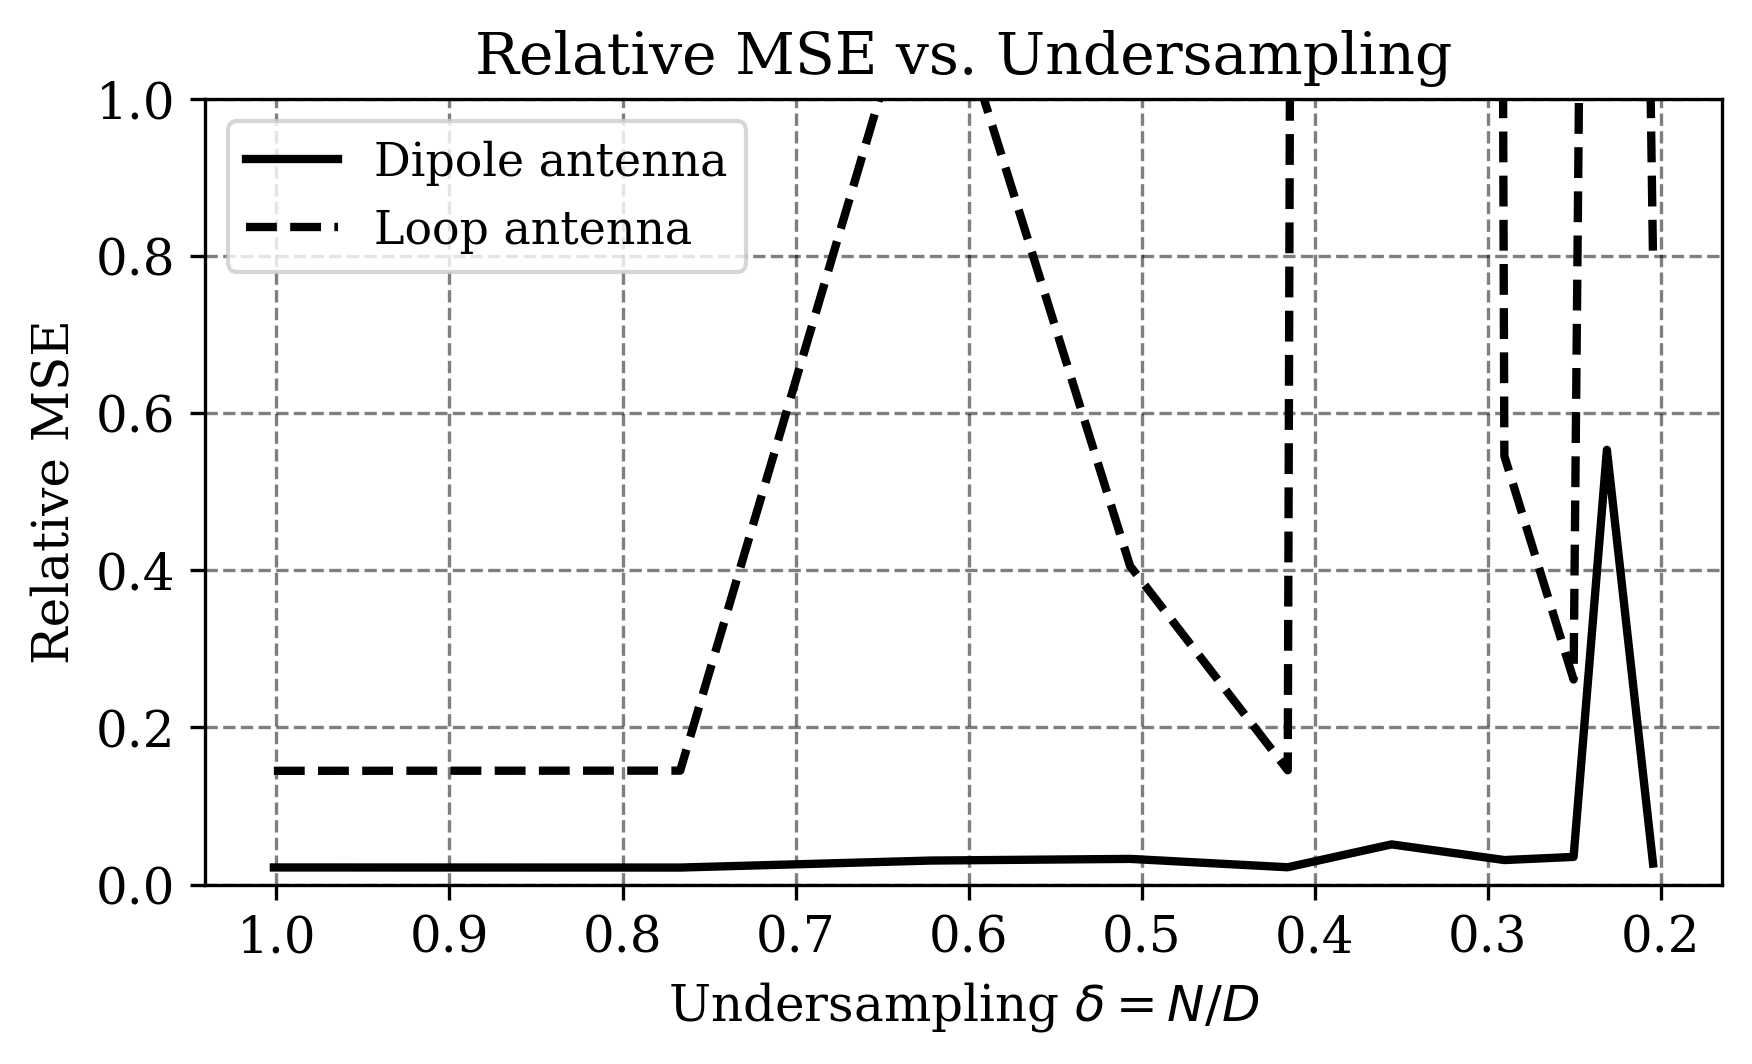
\includegraphics[width=0.95\textwidth]{Figures/delta_vs_mse_ff.png}
            \captionof{figure}{Relative reconstruction error (normalized MSE) as a function of the measurement-to-dimension ratio $\delta = N/D$ for dipole and loop antennas in the far-field configuration.}
            \label{fig:mse_ff}
        \end{column}
    \end{columns}
\end{frame}


\begin{frame}
    \frametitle{NF-to-FF Transformation: Process \& Results}
    \begin{itemize}
    		\item \textbf{Process:}
                \begin{enumerate}
                		\item Simulate near-field and far-field data for dipole and loop antennas.
                    \item Estimate coefficients with SBL from simulated near-field data at $r = 0.5\lambda$.
                    \item Construct field from those coefficients with $\mathbf{F}_{smn}^{(c)}$ evaluated at $r=5\lambda$
                    \item Compute relative MSE between original FF and reconstructed FF
                \end{enumerate}
        \item \textbf{Results:} MSE between far-field simulation results and reconstruction from coefficients very high
        \item \textbf{Further investigation:} Compare coefficients computed from far-field and near-field
    \end{itemize}
\end{frame}

\begin{frame}
    \frametitle{NF-to-FF Transformation: Discrepancies in Coefficients}
    \begin{columns}
        \begin{column}{0.5\textwidth}
            \begin{itemize}
                \item \textbf{Loop Antenna:} Dominant coefficients showed good consistency between near-field and far-field reconstructions.
                \item \textbf{Dipole Antenna:} Showed more significant discrepancies in the estimated coefficients.
                \item This indicates potential issues with the dictionary's ability to represent it sparsely, or numerical precision.
            \end{itemize}
        \end{column}
        \begin{column}{0.5\textwidth}
            \centering
            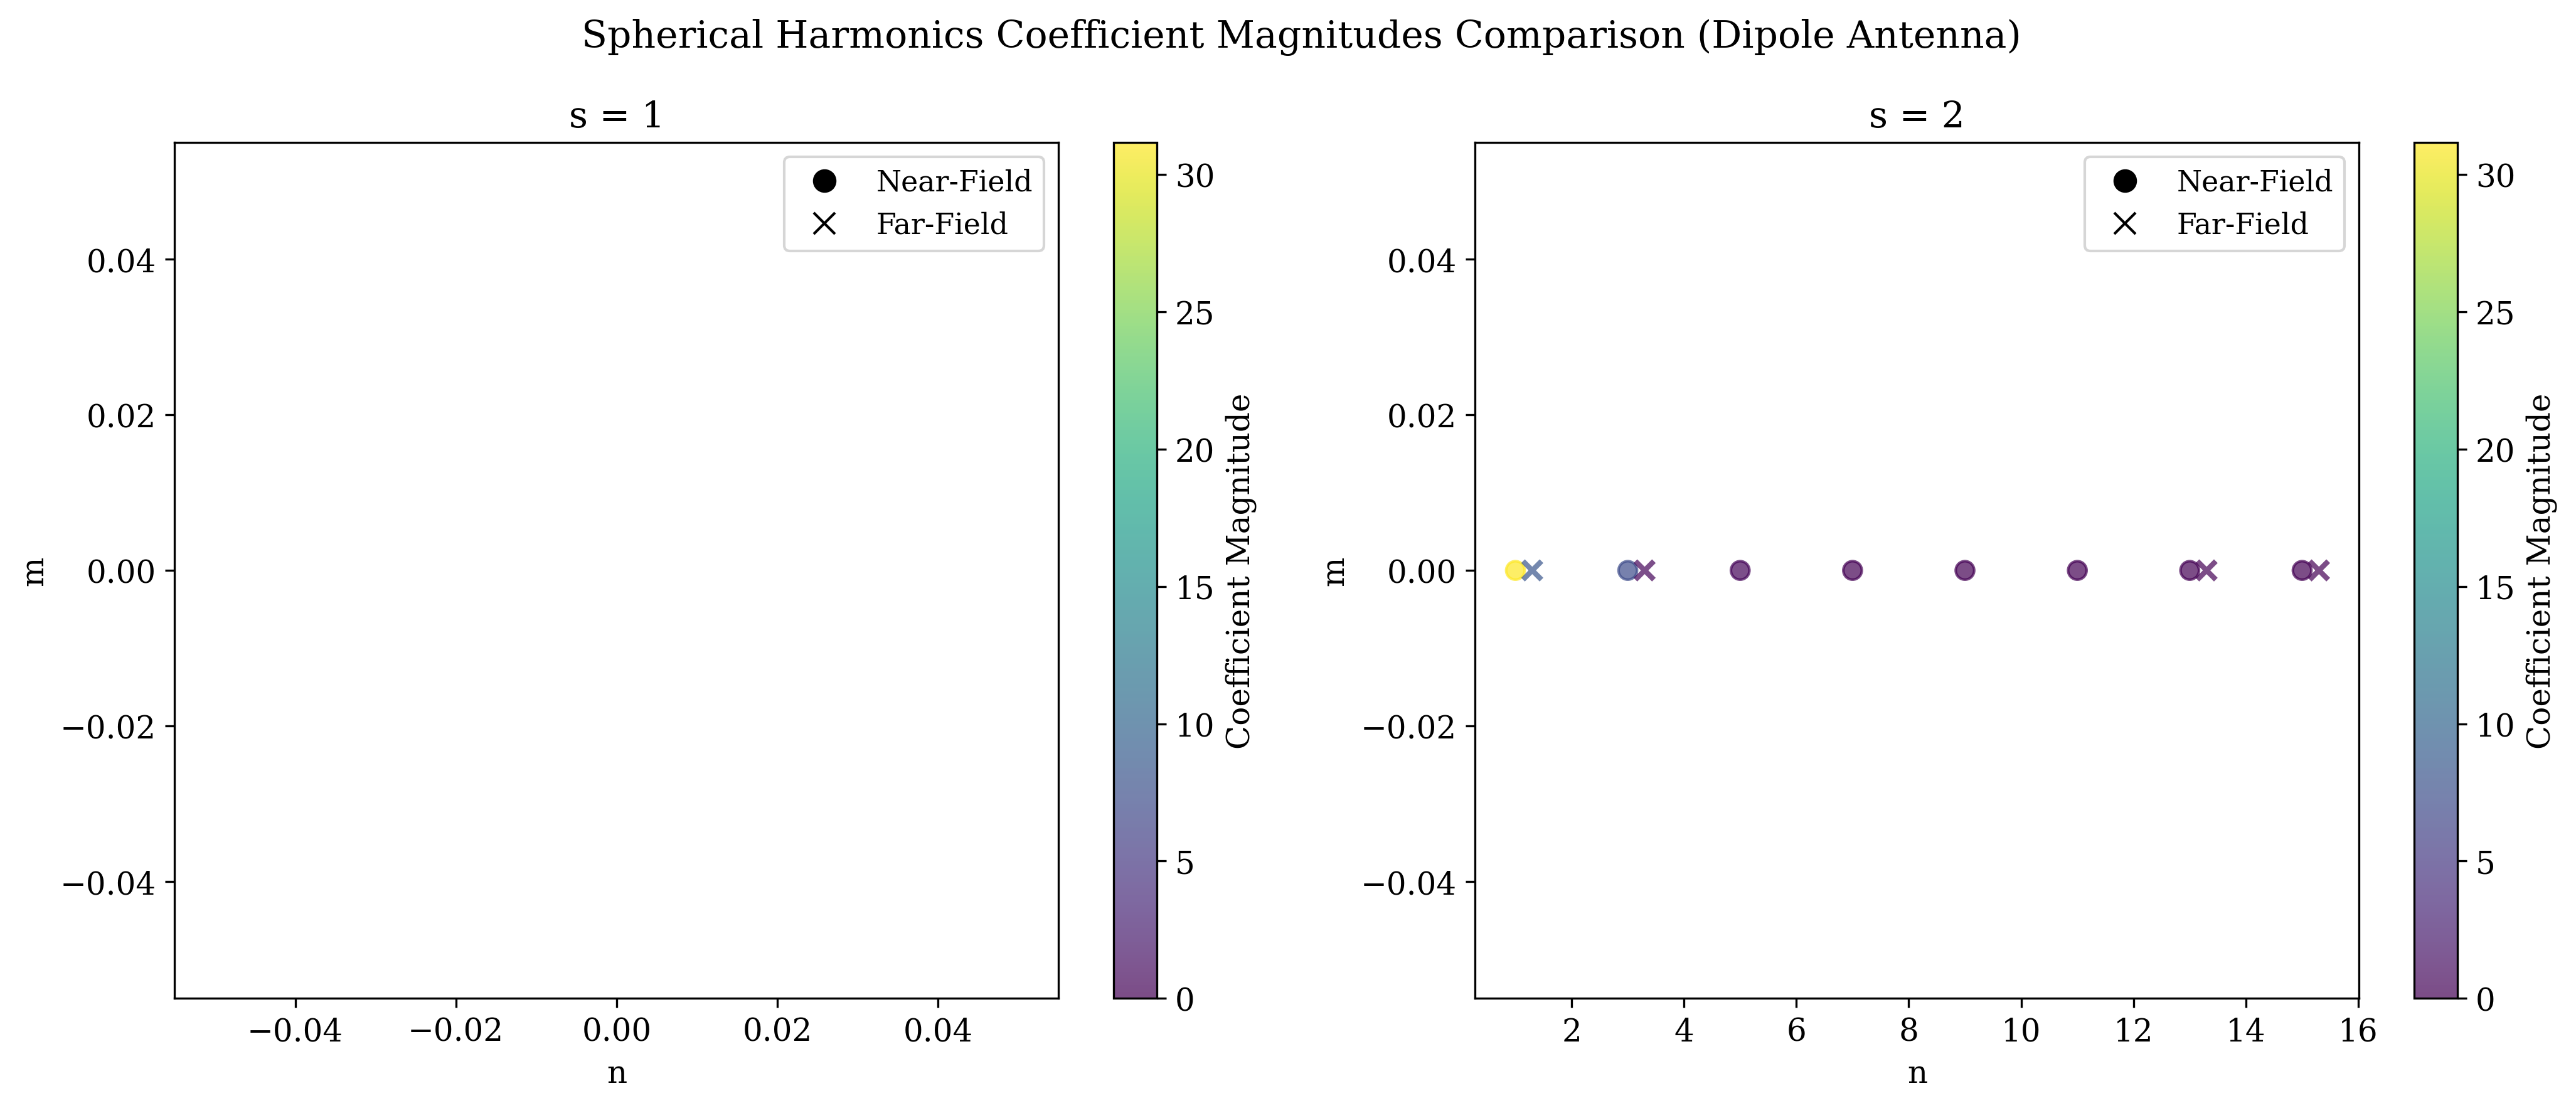
\includegraphics[width=0.95\textwidth]{Figures/dipole_nf_ff_weights.png}
            \captionof{figure}{Comparison of wave coefficients for the dipole antenna: non-zero weights estimated by FML from near-field vs. significant coefficients from far-field.}
            \label{fig:dipole_nfff_weights}
        \end{column}
    \end{columns}
\end{frame}


% --- SECTION: Conclusion ---
\section{Conclusion}

\begin{frame}
    \frametitle{Summary of Achievements}
    \begin{itemize}
        \item \textbf{Theoretical Understanding:} Gained a strong understanding of SBL, different approaches for SBL algorithms and Spherical Wave Expansion.
        \item \textbf{Successful Algorithm Implementation:} Developed robust implementations of SBL algorithms (EM, CoFEM, FML).
        \item \textbf{Application:} Applied Compressive Sensing (specifically Tipping's FML) to the problem of antenna pattern extrapolation from near-field measurements.
        \item \textbf{Key Finding:} Tipping's FML algorithm proved to be the most robust and efficient for the antenna extrapolation problem, particularly with structured Fourier-like dictionary matrices.
    \end{itemize}
\end{frame}

\begin{frame}
    \frametitle{Challenges Encountered}
    \begin{itemize}
        \item \textbf{Numerical Instabilities:} EM algorithm struggled with complex-valued (Fourier) dictionaries.
        \item \textbf{Challenges with SWE via Integration:} The attempt to decompose the electromagnetic field into spherical vector wave components using the classical integration-based method was unsuccessful.
        \item \textbf{Unexpected High Errors:} Attempts at far-field reconstruction from NF data showed higher-than-expected errors even at full sampling, pointing to complexities beyond just undersampling.
        \item \textbf{Coefficient Discrepancies:} Differences in estimated coefficients for certain antenna types (e.g., dipole) between NF and FF estimations.
    \end{itemize}
\end{frame}

\begin{frame}
    \frametitle{Future Work}
    \begin{itemize}
        \item \textbf{Algorithm Optimization:} Further refine and optimize the SBL algorithms for specific antenna models and larger-scale problems.
        \item \textbf{Improved Basis Functions:} Investigate more accurate or specialized spherical wave basis functions to potentially improve reconstruction accuracy.
        \item \textbf{Real-World Validation:} Validate the framework with experimental, real-world antenna measurement data.
        \item \textbf{Advanced Simulations:} Transition to dedicated antenna simulation software (e.g., CST Microwave Studio) for more realistic data generation.
        \item \textbf{Deeper Investigation:} Conduct further research into the inherent physical assumptions and numerical implementation details of SBL for Near-Field to Far-Field Transformation.
    \end{itemize}
\end{frame}

\begin{frame}
    \frametitle{Next Steps}
    \begin{itemize}
    	\item \textbf{Establish Ground Truth via Integration:} Successfully implement SWE using numerical integration to obtain accurate reference coefficients for comparison with SBL results.
    	\item \textbf{Refine SBL Performance:} First ensure reliable reconstruction at $\delta = 1$, then gradually reduce measurements to explore the limits of undersampling robustness.
    	\item \textbf{Sparsity Analysis of SWE Coefficients:} Study the distribution of SWE coefficients across different antenna types to better understand their sparsity structure. This can inform prior design in SBL and improve recovery performance.
    	\item \textbf{Parameter Sensitivity Study:} Investigate how variations in key parameters affect reconstruction accuracy, including:
    	\begin{itemize}
    		\item Radial measurement distance (e.g., $0.5\lambda$ vs. $1\lambda$)
        \item Measurement grid uniformity and angular resolution
        \item Truncation of angular coverage
        \item Noise levels and SNR
        \item Antenna topology (dipole, loop, patch, etc.)
    	\end{itemize}
    \end{itemize}
\end{frame}

\begin{frame}
    \frametitle{Acknowledgments}
    \begin{itemize}
        \item \textbf{Supervisors:}
        \begin{itemize}
            \item Prof. Dirk Slock
            \item Dr. Zilu Zhao
            \item Dr. Fangqing Xiao
        \end{itemize}
        \item \textbf{Tools \& Assistance:}
        \begin{itemize}
            \item Python for all implementations and simulations.
            \item MATLAB for antenna simulation
            \item Large Language Models (LLMs) for debugging, code commenting, and text refinement.
        \end{itemize}
    \end{itemize}
\end{frame}


\end{document}